\documentclass[a4paper,12pt]{article}
\usepackage{cmap}
\usepackage[T2A]{fontenc}
\usepackage[utf8]{inputenc}
\usepackage[russian]{babel}
\usepackage{indentfirst}
\usepackage{graphicx}

\usepackage{geometry}
\geometry{left=3cm}
\geometry{right=2cm}
\geometry{top=2cm}
\geometry{bottom=2cm}

\usepackage[hidelinks]{hyperref}

\usepackage{titletoc}
\newlength{\seclenght}
\settowidth{\seclenght}{7. }
\dottedcontents{section}[\the\seclenght]{}{\the\seclenght}{2mm}
\newlength{\subseclenght}
\settowidth{\subseclenght}{6.2. }
\dottedcontents{subsection}[\the\subseclenght]{}{\the\subseclenght}{2mm}
\newlength{\subsubseclenght}
\settowidth{\subsubseclenght}{6.2.8. }
\dottedcontents{subsubsection}[\the\subsubseclenght]{}{\the\subsubseclenght}{2mm}
\newlength{\pagereflenght}
\settowidth{\pagereflenght}{\pageref{LastPage}}
\contentsmargin{\the\pagereflenght}
\renewcommand{\thesection}{\arabic{section}.}
\renewcommand{\thesubsection}{\thesection\arabic{subsection}.}
\renewcommand{\thesubsubsection}{\thesubsection\arabic{subsubsection}.}
\setcounter{tocdepth}{3}

\usepackage{lastpage}

\begin{document}
\begin{titlepage}
\begin{center}
\hrule\vspace{1em}
\bf Московский государственный технический университет им. Н.Э.\,Баумана\\
Кафедра <<Системы обработки информации и управления>>\\[1em]
\hrule
\end{center}

\vfill

\noindent УТВЕРЖДАЮ:\\[1em]
\underline{\hspace{12em}} Галкин~В.\,А.\\[1em]
<<\underline{\hspace{1em}}>> \underline{\hspace{6.5em}} 2017~г.

\vfill\vfill

\begin{center}
\large Руководство пользователя\\
к~курсовой работе\\
{\Large<<Локальная безадаптерная сеть>>}\\
(вариант №\,26а)\\
по~курсу {\Large<<Сетевые технологии в~АСОИУ>>}
\end{center}

\vfill\vfill\vfill

\begin{tabular*}{\textwidth}{l@{\extracolsep{\fill}}l}
&ИСПОЛНИТЕЛИ:\\[1em]
&\underline{\hspace{12em}} Лещев А.\,О., ИУ5-64\\[1em]
&\underline{\hspace{12em}} Мельников К.\,И., ИУ5-64\\[1em]
&<<\underline{\hspace{1em}}>> \underline{\hspace{6.5em}} 2017~г.\\
\end{tabular*}
 
\vfill

\begin{center}
Москва~--- 2017~г.\\[1em]
\hrule
\end{center}

\end{titlepage}

\setcounter{page}{2}
\tableofcontents
\clearpage

\section{Назначение разработки}
Программа <<Локальная безадаптерная сеть>> позволяет передавать файлы по~локальной сети с~возможностью докачки после восстановления прерванной связи, состоящей из~двух персональных компьютеров, соединённых через интерфейс RS-232C нуль-модемным кабелем.

\section{Условия выполнения программы}
Для~работы программы требуются два персональных компьютера, поддерживающие операционную систему Microsoft Windows версии~10, работающие под~её управлением и соединённые нуль-модемным кабелем через интерфейс RS-232C или иным каналом, эмулирующим данный интерфейс. Вместо персональных компьютеров допускается использование виртуальных машин под~управлением гипервизора Oracle VM VirtualBox, соединённых виртуальным нуль-модемным кабелем.

Также требуется оператор (пользователь), имеющий базовые знания о~работе с~персональным компьютером и операционной системой Microsoft Windows версии~10.

\section{Выполнение программы}
\subsection{Установка программы}
Для~установки программы следует скопировать файл \texttt{iu5nt.exe} на~персональный компьютер.

\subsection{Удаление программы}
Для~удаления программы следует удалить установленный файл \texttt{iu5nt.exe} с~персонального компьютера.

\subsection{Запуск программы}
Для~запуска программы следует запустить предварительно установленный файл \texttt{iu5nt.exe}. При~этом откроется главное окно программы (рисунок~\ref{window}).
\begin{figure}
\centering
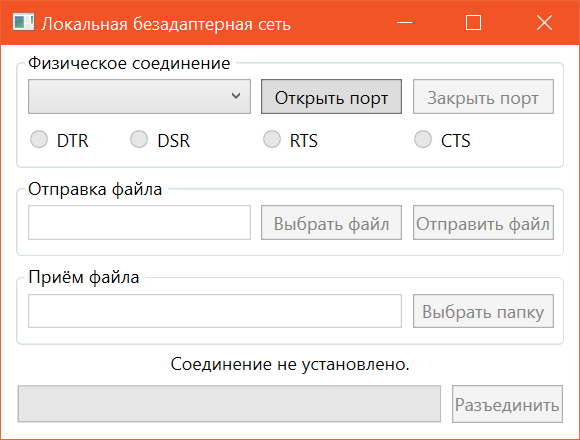
\includegraphics{window.png}
\caption{Главное окно программы.}\label{window}
\end{figure}

\subsection{Работа с~программой}
После запуска программы открывается главное окно программы (рисунок~\ref{window}).

При~нажатии на~выпадающий список открывается список с~доступными COM-портами (рисунок~\ref{list}). Выбранный порт будет использоваться для~соединения.
\begin{figure}
\centering
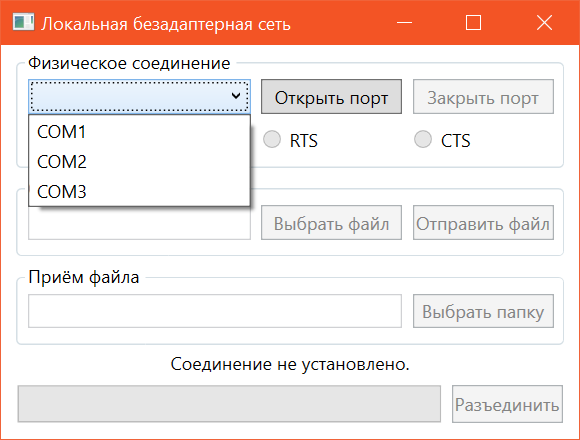
\includegraphics{list.png}
\caption{Выпадающий список доступных COM-портов.}\label{list}
\end{figure}

Нажатие на~кнопку <<Открыть порт>> позволяет установить физическое соединение (рисунок~\ref{open}). При~этом разблокируется возможность выбора файла для~отправки и папки для~приёма файла и выводится информационное сообщение <<Физическое соединение открыто>>.
\begin{figure}
\centering
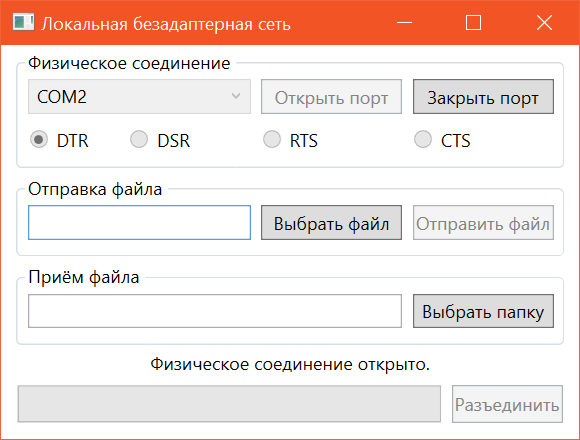
\includegraphics{open.png}
\caption{Окно программы после открытия физического соединения.}\label{open}
\end{figure}
При~открытии порта на~другом компьютере устанавливается физическое соединение, что отображается индикатором DSR.
\begin{figure}
\centering
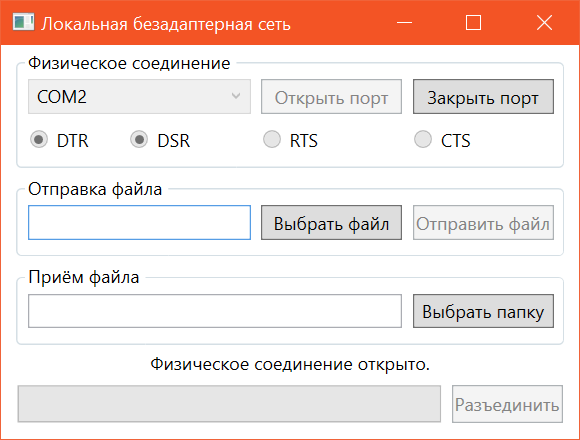
\includegraphics{dsr.png}
\caption{Окно программы после установки физического соединения.}\label{dsr}
\end{figure}

Нажатие на~кнопку <<Выбрать файл>> позволяет выбрать файл~для отправки. При~её нажатии открывается стандартное диалоговое окно выбора файла (рисунок~\ref{file}).
\begin{figure}
\centering
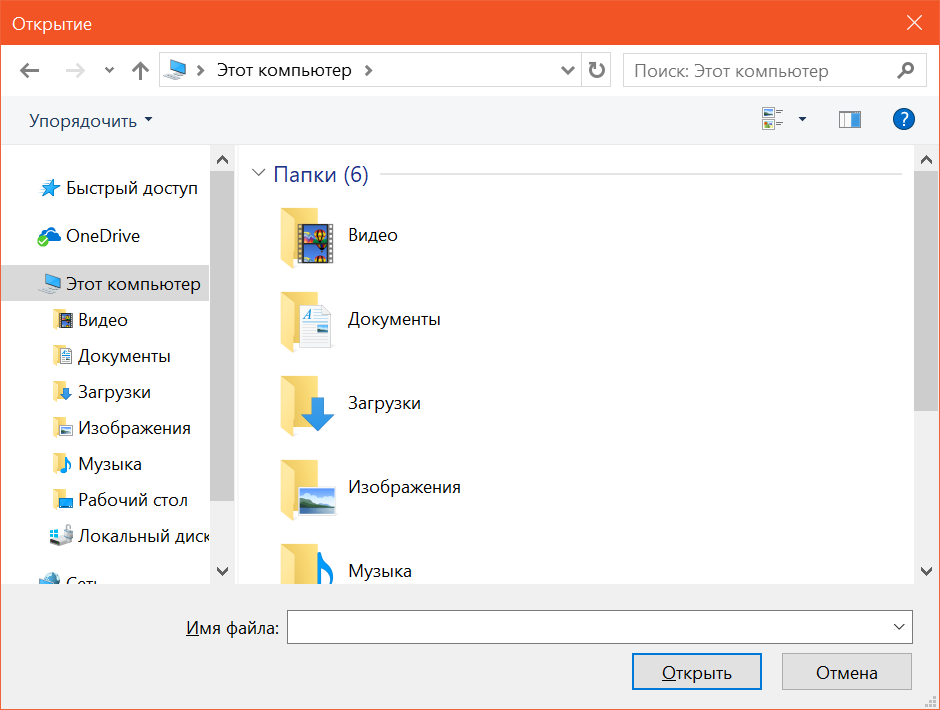
\includegraphics[width=\linewidth]{file.png}
\caption{Окно выбора файла для~отправки.}\label{file}
\end{figure}
После выбора файла разблокируется кнопка <<Отправить файл>> (рисунок~\ref{send}).
\begin{figure}
\centering
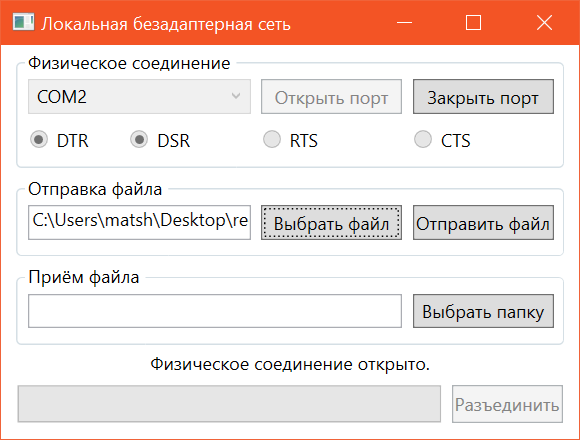
\includegraphics{send.png}
\caption{Окно программы после выбора файла.}\label{send}
\end{figure}

Нажатие на~кнопку <<Выбрать папку>> позволяет выбрать папку, в~которую будут сохраняться принятые файлы. При~её нажатии открывается стандартное диалоговое окно выбора папки (рисунок~\ref{folder}).
\begin{figure}
\centering
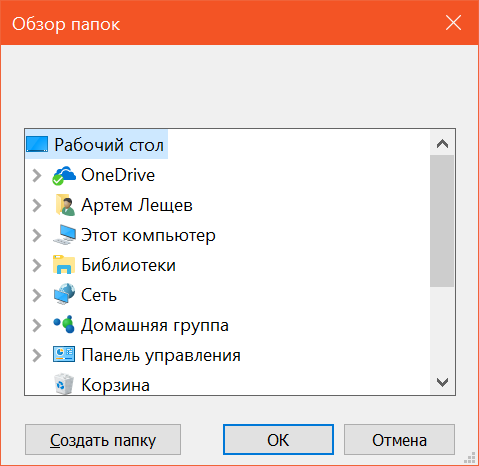
\includegraphics{folder.png}
\caption{Окно выбора папки для~приёма файлов.}\label{folder}
\end{figure}
После выбора папки на~другом компьютере (при~установленной физической связи) загорается индикатор CTS (рисунок~\ref{cts}).
\begin{figure}[!h]
\centering
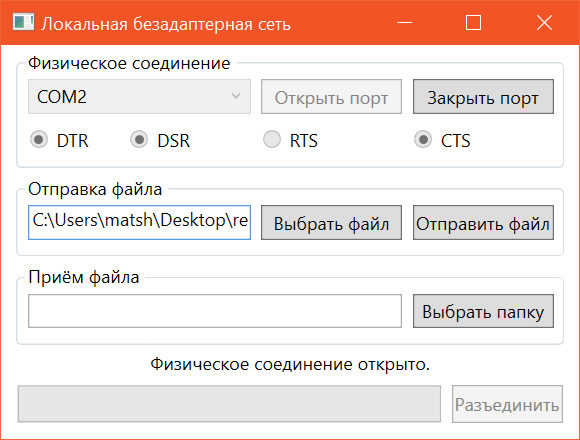
\includegraphics{cts.png}
\caption{Окно программы другого компьютера после выбора папки.}\label{cts}
\end{figure}

После выбора папки на~принимающем компьютере можно нажать кнопку <<Отправить файл>> в~передающей программе, чтобы отправить выбранный файл. Во~время передачи файла будет заполняться индикатор передачи файла (рисунок~\ref{progress}).
\begin{figure}
\centering
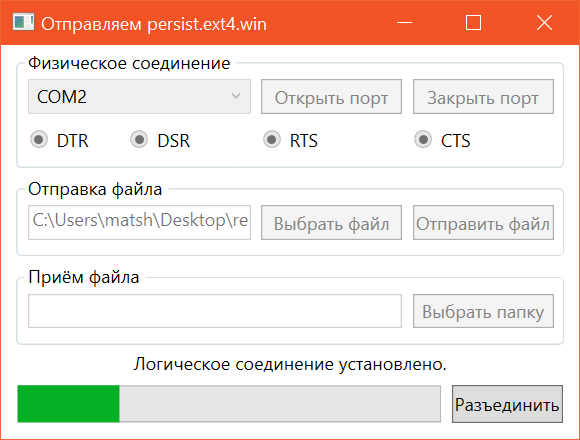
\includegraphics{progress.png}
\caption{Процесс передачи файла.}\label{progress}
\end{figure}

После успешной передачи будет отображено соответствующее сообщение на~каждом из~компьютеров (рисунок~\ref{fin}).
\begin{figure}
\centering
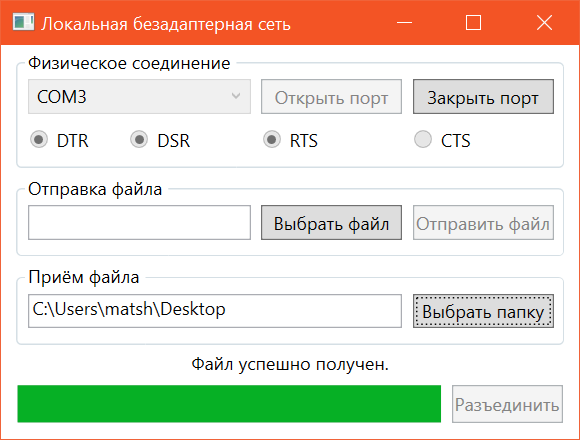
\includegraphics{fin.png}
\caption{Окно принимающей программы после приёма файла.}\label{fin}
\end{figure}

\section{Устранение неполадок}
При~работе программы может возникнуть ряд ошибок. Необходимо выполнить следующие действия при~возникновении ошибки:
\begin{itemize}
\item <<\texttt{Сначала необходимо выбрать порт.}>>~--- выберите порт перед его открытием.
\item <<\texttt{Принимающая сторона не~готова к~логическому соединению.}>>~--- убедитесь, что компьютеры соединены правильно и на~принимающей стороне выбрана папка для~приёма файлов.
\item <<\texttt{Логическое соединение потеряно.}>>~--- проверьте соединение компьютеров.
\item <<\texttt{Получен повреждённый пакет.}>>~--- проверьте качество соединения компьютеров и правильность выбора порта.
\item <<\texttt{Получен неизвестный пакет.}>>~--- проверьте правильность выбора порта.
\end{itemize}

\end{document}